% 1405/5/4
% H. Behrouz 
% Email : Texlivegroup@gmail.com


\documentclass{beamer}
% 1405/5/4
% H. Behrouz 
% Email : Texlivegroup@gmail.com



% بعد از هر تغییر در این قسمت کلید Ctrl+S را بزنید و اجرا و مشاهده pdf فقط در فایل Slide.tex   می‌باشد.


% در این قسمت می‌توانید پکیج‌های مورد نیاز را اضافه کنید.
\usepackage{amsmath,amssymb,amsfonts}
\usepackage{mathtools}
\usepackage{xcolor} 
\usepackage{array}
\usepackage{multirow}
\usepackage{tikz} 
\usepackage{graphicx}
\usepackage{subfigure}
\usepackage{listings}
\usepackage{ragged2e}
\usepackage{mathtools}
\usepackage{float}
\usepackage{caption}
\usepackage{pifont}
\usepackage{tasks}
\usepackage{verbatim}





% انتخاب تم برای اسلاید 
\usetheme{Madrid}
%\usetheme{AnnArbor}
%\usetheme{CambridgeUS}
%\usetheme{Copenhagen}
%\usetheme{Ilmenau}
%\usetheme{Warsaw}


\usefonttheme[stillsansserifmath]{serif}


% به جای blue  در سطر ۳۱  می‌توانید هر یک از رنگ زیر را استفاده کنید
% black, blue, brown, cyan, darkgray, gray, green, lightgray, lime, magenta, olive, orange, pink, purple, red, teal, violet, white, yellow
\usecolortheme[named=blue]{structure}
\setbeamercovered{transparent}



% تعریف فونت 
\usepackage{xepersian}
\settextfont{Yas}
\setdigitfont{Yas}
\defpersianfont\nas[Scale=1.5]{IranNastaliq}


% دستور لوگو
\newcommand{\nologo}{\setbeamertemplate{logo}{logo}}


% سه خط دستور زیر در صورت فعال نبودن  شماره اسلاید فعال کنید
%\expandafter\def\expandafter\insertshorttitle\expandafter{%
%\insertshorttitle\hfill%
%\inserttotalframenumber\,/\,\insertframenumber}


% دستور ایجاد شماره برای  عکس و جدول
\setbeamertemplate{caption}[numbered]












% در قسمت زیر مشخصات خود را وارد کنید و اگر طبق تم انتخابی فاصله‌ها کم یا زیاد شد می‌توانید عدد پیش‌فرض 0.7cm را تغییر دهید.
\title[
دانشگاه تبریز
]{
عنوان اسلاید
}
\author[
نام دانشجو
]{\textbf{
نام دانشجو
\\[0.7cm]
استاد راهنما
\\[0.7cm]
دکتر ...
\\[0.7cm]
}} 
\institute[دانشگاه تبریز]{
\textit{\textbf{
دانشگاه تبریز
}}
\\[0.5cm]
}
\date{
  تیر
$1405$ 
}
\begin{document}
% اسلاید زیر برای اولین اسلاید یعنی بسم‌الله بوده و می‌توانید در صورت نیاز با عکس بسم‌الله دیگری جایگزین شود نام عکس هم باید طبق عکس جدید در زیر تغییر کند.  حتما عکس جدید را داخل پوشه کپی کرده و در صورت نیاز تغییر نام بدید.
\begin{frame}[plain]
\begin{figure}
\centering

\includegraphics[width=0.7\linewidth]{besm}
\end{figure}

\end{frame}
\begin{frame}
\centering
\titlepage 
\end{frame}
% دستور زیر برای قرار دادن لوگوی دانشگاه می‌باشد، در صورت قرار دادن لوگوی خود اگر عکس برزگ یا کوچک بود عدد پیش scale را تغییر دهید.  حتما عکس جدید را داخل پوشه کپی کرده و  تغییر نام بدید به  logo
\logo{
\includegraphics[scale=.2]{logo}}

% در اسلاید زیر فهرست مطالب خود را وارد کنید.
\begin{frame}{فهرست}
\begin{tasks}
\task[1.]
\textbf{
چکیده
}
\vspace{0.5cm}
\task[2.]
\textbf{
عنوان فصل اول 
 }
\vspace{0.5cm}
\task[3.]
\textbf{
عنوان فصل دوم 
}
\vspace{0.5cm}
\task[4.]
\textbf{
عنوان فصل سوم 
}
\vspace{0.5cm}
\task[5.]
\textbf{
مراجع
}
\end{tasks}
\end{frame}



\begin{frame}
\frametitle{}
\framesubtitle{}
\begin{block}{چکیده}
\justifying	
لطفا از نمونه اسلایدهای که ایجاد شده استفاده کنید  و همچنین توضیحاتی که در کامنت‌ها در طول اسلاید وجود دارد توجه کنید.
\end{block}	
\end{frame}




% دستور section زیر را می‌توان برای عنوان کوتاه برای تم Ilmenau فعال کنید که با دو بار اجرا اعمال می‌شود.
%\section[فصل ۱]{}
\begin{frame}
\begin{huge}
\begin{center}
\textbf{
فصل 
1
}
\\[1.5cm]

\textbf{
عنوان فصل اول خود را وارد کنید... 
}
\end{center}
\end{huge}
\end{frame}


% نمونه اسلاید محیط تعریف و قضیه
\begin{frame}
\frametitle{}
\framesubtitle{}
\begin{block}{تعریف}
منظور از یک گروه لی، منیفلدی هموار مانند
$ G $
می‌باشد به‌طوری که دارای ساختار جبری گروه بوده و دو نگاشت ضرب و وارون‌ساز 
$ m:G\times G \longrightarrow G $
و
$ i:G \longrightarrow G $
که با ضابطه‌های
\begin{equation}
m\left( g,h\right) =g\cdot h, \qquad i(g)=g^{-1}
\end{equation}
تعریف می‌شوند، هموار باشند.
\end{block}
\begin{block}{قضیه}
فرض کنید که 
$ G $ 
یک گروه‌لی همبند با جبرلی 
$ \mathfrak{g} $
باشد. و دراین‌ صورت برای هر 
$ g \in G $
، \,
$ V_{1},\cdots,V_{k}\in \mathfrak{g} $
وجود دارد به طوریکه
\begin{equation*}
g=\exp(V_{1})\circ \cdots \circ \exp (V_{k}).
\end{equation*}
\end{block}	
\end{frame}




% نمونه محیط ایجاد ایتم‌بندی
\begin{frame}
\frametitle{عنوان فصل }
\framesubtitle{عنوان بخش}
\begin{block}{محیط ایتم}
\justifying	
نمونه محیط ایتم‌بندی
\begin{tasks}
\task[1.]
 ایتم اول
\task[2.] 
ایتم دوم
\task[3.] 
ایتم دوم
\end{tasks}
پایان محیط ایتم بندی
\end{block}	
\end{frame}




% نمونه محیط ایجاد ایتم‌بندی
\begin{frame}
\frametitle{عنوان فصل }
\framesubtitle{عنوان بخش}
\begin{block}{محیط ایتم دو ستونی}
\justifying	
نمونه محیط 
\begin{tasks}(2)
\task[1.]
 ایتم اول
\task[2.]  
ایتم دوم
\task[3.]
ایتم سوم
\task[4.]
ایتم چهارم
\end{tasks}
ایتم‌بندی
\end{block}	
\end{frame}







% نمونه محیط ایجاد ایتم‌بندی
\begin{frame}
\frametitle{عنوان فصل }
\framesubtitle{عنوان بخش}
\begin{block}{محیط ایتم}
\justifying	
تغییر شماره گذاری، محیط ایتم:
\begin{tasks}
\task[\ding{182}]
 ایتم اول
\task[\ding{173}]  
ایتم دوم
\task[$\bullet$]
ایتم دوم
\end{tasks}
می‌توان از همه نمادها که در لاتک تعریف شده استفاده کنید.
\end{block}	
\end{frame}


% نمونه محیط وارد کردن کد برنامه‌نویسی و حذف لوگو فقط در این اسلاید
{\nologo
\begin{frame}[fragile]
\frametitle{عنوان فصل }
\framesubtitle{عنوان بخش}
نمونه اسلاید برای وارد کردن کد برنامه‌نویسی
\begin{latin}
\begin{verbatim}
import matplotlib.pyplot as plt
import numpy as np
import matplotlib as mpl
np.random.seed(19680801) 
data = {'a': np.arange(50),
'c': np.random.randint(0, 50, 50),
'd': np.random.randn(50)}
data['b'] = data['a'] + 10 * np.random.randn(50)
data['d'] = np.abs(data['d']) * 100
fig, ax = plt.subplots(figsize=(5, 2.7),
 layout='constrained')
ax.scatter('a', 'b', c='c', s='d', data=data)
ax.set_xlabel('entry a')
ax.set_ylabel('entry b')
\end{verbatim}
\end{latin}
\end{frame}
}





% نمونه اسلاید وارد کردن عکس  حتما عکس جدید را داخل پوشه کپی کرده و در صورت نیاز تغییر نام بدید.
\begin{frame}
\frametitle{عنوان فصل }
\framesubtitle{عنوان بخش}
\begin{block}{}
\justifying	
نمونه کد عکس داخل محیط block
\begin{figure}
\centering
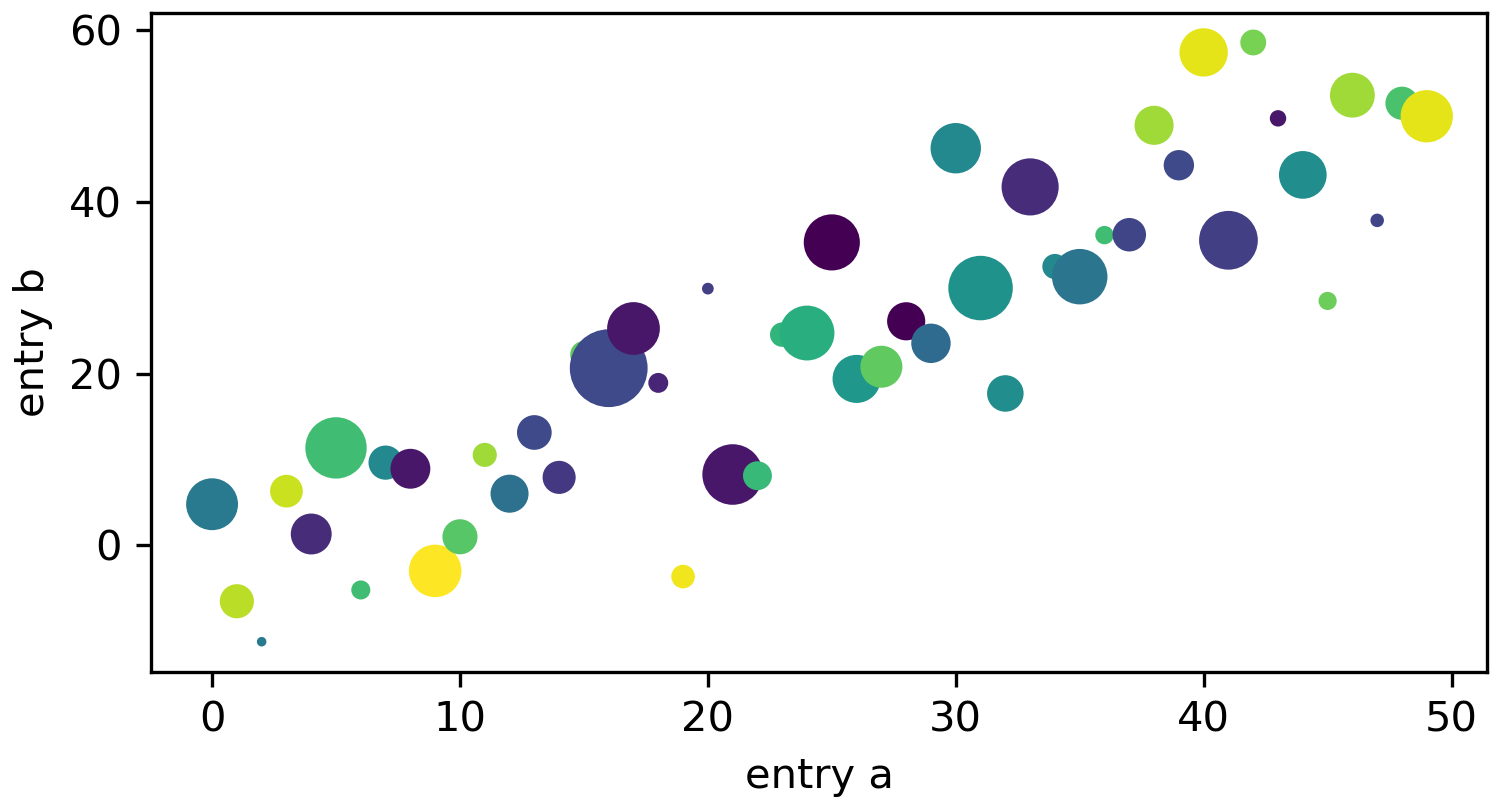
\includegraphics[width=0.7\linewidth]{1}
\caption{
\centering
برای زیبایی در صورت طولانی بودن کپشن عکس از دستور centering مانند این نمونه داخل محیط کپشن اضافه کنید  
}
\label{fig:1}
\end{figure}
\end{block}	
\end{frame}


% نمونه اسلاید وارد کردن عکس  حتما عکس جدید را داخل پوشه کپی کرده و در صورت نیاز تغییر نام بدید.
\begin{frame}
\frametitle{عنوان فصل }
\framesubtitle{عنوان بخش}
\justifying	
نمونه کد عکس بدون محیط block
\begin{figure}
\centering
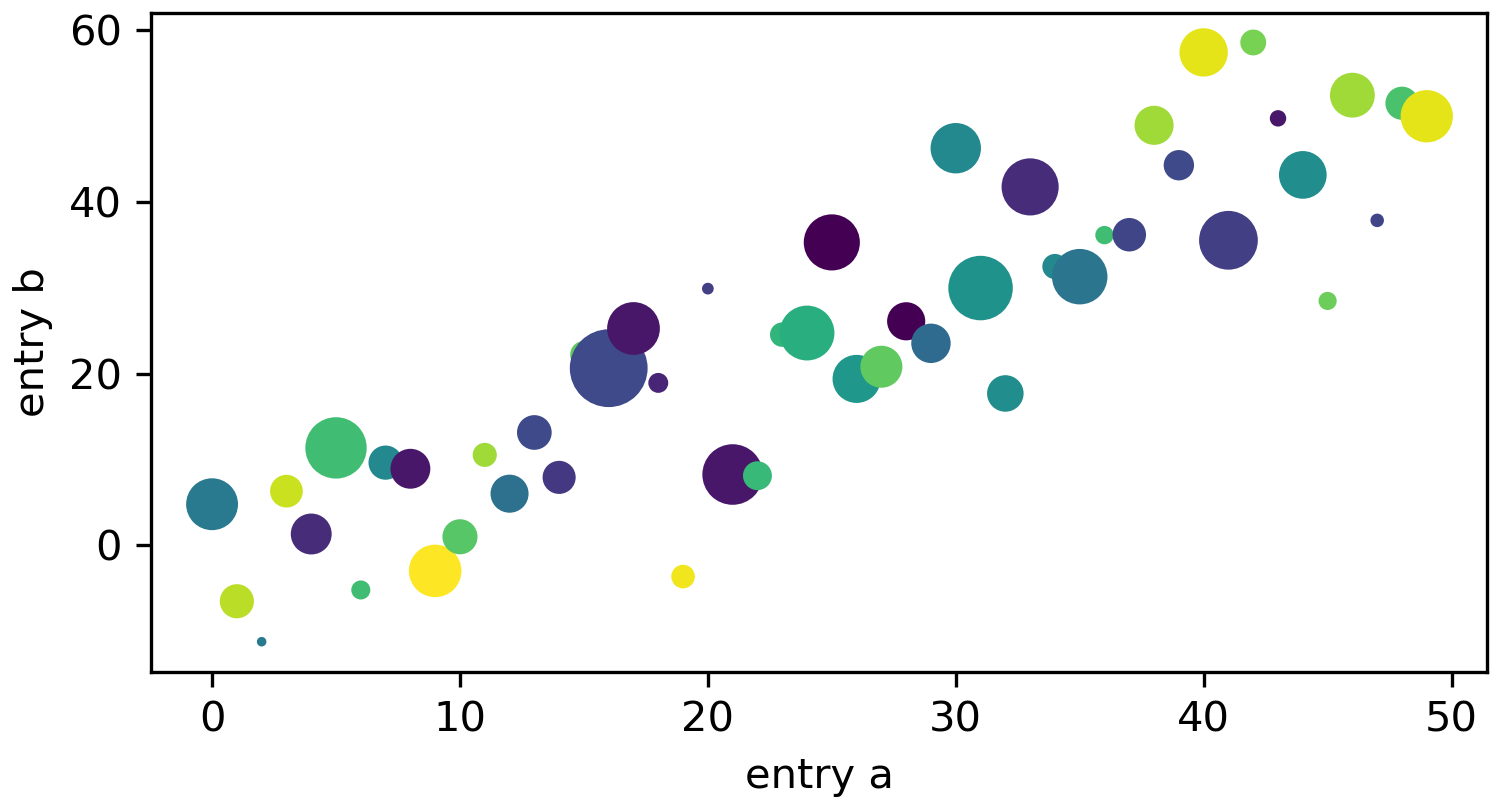
\includegraphics[width=0.7\linewidth]{1}
\caption{
\centering
برای زیبایی در صورت طولانی بودن کپشن عکس از دستور centering مانند این نمونه داخل محیط کپشن اضافه کنید  
}
\label{fig:2}
\end{figure}
	
\end{frame}



% نمونه اسلاید وارد کردن جدول
\begin{frame}
\frametitle{عنوان فصل }
\framesubtitle{عنوان بخش}
\begin{block}{نمونه جدول داخل محیط بلوک}
\justifying	
\begin{table}[!h]
\centering
\begin{tabular}{|cccccc|c|}
\hline
$ Y_{6} $ & $ Y_{5} $ & $ Y_{4} $ & $ Y_{3} $ & $ Y_{2} $ & $ Y_{1} $ &   [,]  \\
\hline
$ -Y_{5} $ & $ Y_{6} $ &  0 & $ -Y_{2} $ & $ Y_{3} $  & 0 & $ Y_{1} $ \\
0 & $ Y_{4} $ & $ -Y_{5} $ & $ Y_{1} $  & 0 & $ -Y_{3} $ & $ Y_{2} $ \\
$ Y_{4} $ &  0 & $ -Y_{6} $  & 0 & $ -Y_{1} $ & $ Y_{2} $ & $ Y_{3} $  \\
$ Y_{3} $ & $ Y_{2} $  & 0 & $ Y_{6} $ & $ Y_{5} $ & 0 & $ Y_{4} $  \\
$ -Y_{1} $  & 0 & $ -Y_{2} $  & 0 & $ -Y_{4} $ & $ -Y_{6} $ & $ Y_{5} $  \\
0 & $ Y_{1} $ & $ -Y_{3} $ & $ -Y_{4} $  & 0 & $ Y_{5} $ &  $ Y_{6} $  \\
\hline
\end{tabular} 
\caption{\centering
برای زیبایی در  جدول‌ها اگر کپشن خیلی طولانی است مانند این نمونه دستور centering را داخل کپشن قرار دهید
}
\label{tab:my-table-1}
\end{table}
\end{block}	
\end{frame}


% نمونه اسلاید وارد کردن جدول
\begin{frame}
\frametitle{عنوان فصل }
\framesubtitle{عنوان بخش}
\justifying	
نمونه جدول بدون محیط بلوک
\begin{table}[!h]
\centering
\begin{tabular}{|cccccc|c|}
\hline
$ Y_{6} $ & $ Y_{5} $ & $ Y_{4} $ & $ Y_{3} $ & $ Y_{2} $ & $ Y_{1} $ &   [,]  \\
\hline
$ -Y_{5} $ & $ Y_{6} $ &  0 & $ -Y_{2} $ & $ Y_{3} $  & 0 & $ Y_{1} $ \\
0 & $ Y_{4} $ & $ -Y_{5} $ & $ Y_{1} $  & 0 & $ -Y_{3} $ & $ Y_{2} $ \\
$ Y_{4} $ &  0 & $ -Y_{6} $  & 0 & $ -Y_{1} $ & $ Y_{2} $ & $ Y_{3} $  \\
$ Y_{3} $ & $ Y_{2} $  & 0 & $ Y_{6} $ & $ Y_{5} $ & 0 & $ Y_{4} $  \\
$ -Y_{1} $  & 0 & $ -Y_{2} $  & 0 & $ -Y_{4} $ & $ -Y_{6} $ & $ Y_{5} $  \\
0 & $ Y_{1} $ & $ -Y_{3} $ & $ -Y_{4} $  & 0 & $ Y_{5} $ &  $ Y_{6} $  \\
\hline
\end{tabular} 
\caption{\centering
برای زیبایی در  جدول‌ها اگر کپشن خیلی طولانی است مانند این نمونه دستور centering را داخل کپشن قرار دهید
}
\label{tab:my-table-2}
\end{table}
\end{frame}





% نمونه ایجاد بلوک با رنگ دلخواه، هر یک از رنگ‌های black, blue, brown, cyan, darkgray, gray, green, lightgray, lime, magenta, olive, orange, pink, purple, red, teal, violet, white, yellow را می‌توانید جایگذین رنگ‌های پیش‌فرض تعریف شده  در دستور زیر کنید.
\begin{frame}
\frametitle{}
\framesubtitle{}
\setbeamercolor{block body}{bg=yellow!20!white,fg=blue}
\setbeamercolor{block title}{fg=purple, bg=red!40}
\begin{block}{نمونه بلوک با رنگ دلخواه}
\justifying	
منظور از یک گروه لی، منیفلدی هموار مانند
$ G $
می‌باشد به‌طوری که دارای ساختار جبری گروه بوده و دو نگاشت ضرب و وارون‌ساز 
$ m:G\times G \longrightarrow G $
و
$ i:G \longrightarrow G $
که با ضابطه‌های
\begin{equation}
m\left( g,h\right) =g\cdot h, \qquad i(g)=g^{-1}
\end{equation}
تعریف می‌شوند، هموار باشند.
\end{block}
\end{frame}







% اسلاید اضافه کردن مراجع 
\nologo
\begin{frame}[allowframebreaks]
\begin{center}
\textbf{{\large مراجع}}
\end{center}
\setbeamertemplate{bibliography item}{\insertbiblabel}
\begin{latin}
\begin{thebibliography}{99} 


\bibitem{R1}
 Anco S., Bluman G., Direct construction of conservation laws, Phys. Rev. Lett., 78 (1997), 2869-2873.

\bibitem{R2}
 Anco S., Bluman G., Direct construction method for conservation laws of partial differential equations Part II: General treatment,
Europ. J. Appl. Math., 13 (2002), 567-585.
 
\bibitem{R3}
Bluman G., Cheviakov A. F., Anco S., Application of symmetry methods to partial differential equations, Springer, 2010.



\end{thebibliography}
\end{latin}

\end{frame}



% اسلاید تشکر و قدر دانی می‌توانید عکس دلخواه خود را جایگزین کنید حتما عکس جدید را داخل پوشه کپی کرده و در صورت نیاز تغییر نام بدید.
\usebackgroundtemplate{
\includegraphics[width=\paperwidth]{tashkor.jpg}}
\begin{frame}[plain]
\end{frame}








\end{document}
